\section{Mitigation Strategies}
\label{sec:mitigation}

The distribution-shift analysis showed that the Graph-Temporal model
increases the width of its prediction intervals during high-congestion
periods, but this adaptation is not sufficient to preserve the desired
coverage, particularly at the 60-minute forecasting horizon. This section
investigates a post-hoc calibration strategy designed to improve the
reliability of the probabilistic forecasts without retraining the forecasting
model. A second, training-based mitigation strategy is subsequently discussed
as a possible extension.

\subsection{Conformalized Quantile Regression}
\label{subsec:cqr}

Conformalized Quantile Regression (CQR) was applied as a post-hoc calibration
procedure to the prediction intervals produced by the trained Graph-Temporal
model. The method uses the validation set as a calibration set and adjusts
the lower and upper predicted quantiles according to their observed
nonconformity with respect to the ground truth. The median prediction is left
unchanged, so the procedure affects uncertainty estimation without modifying
the point forecast.

For each valid calibration target $y_i$, with predicted lower and upper
quantiles $\hat{q}_{0.1,i}$ and $\hat{q}_{0.9,i}$, the nonconformity score is
defined as

\begin{equation}
    s_i =
    \max\left(
        \hat{q}_{0.1,i} - y_i,\,
        y_i - \hat{q}_{0.9,i}
    \right).
    \label{eq:cqr_score}
\end{equation}

The score measures how far an observation lies outside the predicted
interval. Observations already contained within the interval produce
non-positive scores, whereas positive scores quantify the amount by which
the interval fails to cover the target.

The calibration scores are then used to determine how much the original
prediction intervals should be enlarged. Since the target coverage is 80\%,
the desired miscoverage level is $\alpha=0.2$. Let $n_{\mathrm{cal}}$ denote
the number of valid calibration scores. The correction $\hat{s}$ is selected
as the empirical quantile of the calibration scores at level

\begin{equation}
    q =
    \frac{\left\lceil (n_{\mathrm{cal}}+1)(1-\alpha) \right\rceil}
         {n_{\mathrm{cal}}},
    \label{eq:cqr_quantile_level}
\end{equation}

and therefore

\begin{equation}
    \hat{s}
    =
    Q_q\left(\{s_i\}_{i=1}^{n_{\mathrm{cal}}}\right).
    \label{eq:cqr_correction}
\end{equation}

Intuitively, $\hat{s}$ represents the amount by which the original interval
must be expanded so that approximately 80\% of the calibration targets are
covered.

The calibrated prediction interval for a test observation is obtained by
expanding both bounds by this correction,

\begin{equation}
    \left[
        \hat{q}_{0.1,i} - \hat{s},
        \;
        \hat{q}_{0.9,i} + \hat{s}
    \right].
    \label{eq:cqr_interval}
\end{equation}

The procedure is performed separately for each forecasting horizon, allowing
the calibration correction to reflect the different uncertainty levels at
15, 30, and 60 minutes. All calibration quantities are estimated exclusively
from the validation partition and are subsequently kept fixed during test
evaluation. Therefore, no test targets are used to determine the conformal
correction.

CQR therefore provides a lightweight mitigation strategy: it does not alter
the Graph-Temporal architecture, its learned parameters, or its median
forecast, but only recalibrates the predicted uncertainty intervals. This
makes it particularly suitable for the failure mode identified in
Section~\ref{sec:distribution_shift}, where the model already reacts to
high-congestion conditions by increasing interval width, but still exhibits
residual undercoverage.


\subsubsection{Calibration Results}
\label{subsubsec:cqr_results}

The effect of CQR is evaluated by comparing the empirical coverage and
prediction interval width before and after calibration. Table~\ref{tab:cqr_results}
reports the results for the complete test set and separately for normal and
high-congestion conditions.

\begin{table}[t]
    \centering
    \caption{Empirical coverage before and after CQR calibration under
    overall, normal, and high-congestion test conditions.}
    \label{tab:cqr_results}
    \begin{tabular}{llrr}
        \toprule
        Condition & Horizon & Before CQR (\%) & After CQR (\%) \\
        \midrule
        Overall
        & 15 min & 78.44 & 80.24 \\
        & 30 min & 78.22 & 80.14 \\
        & 60 min & 78.13 & 79.96 \\
        \midrule
        Normal
        & 15 min & 78.4 & 80.27 \\
        & 30 min & 78.3 & 80.23 \\
        & 60 min & 78.3 & 80.21 \\
        \midrule
        High congestion
        & 15 min & 78.74 & 79.89 \\
        & 30 min & 77.87 & 79.07 \\
        & 60 min & 75.81 & 77.04 \\
        \bottomrule
    \end{tabular}
\end{table}

As shown in Table~\ref{tab:cqr_results}, CQR effectively corrects the mild
undercoverage observed on the complete test distribution. Empirical coverage
increases from 78.44\%, 78.22\%, and 78.13\% to 80.24\%, 80.14\%, and
79.96\% at the 15, 30, and 60-minute horizons, respectively. The calibrated
intervals are therefore very close to the nominal 80\% coverage level across
all three forecasting horizons.

A similar behavior is observed under normal traffic conditions, where
coverage after calibration reaches 80.27\%, 80.23\%, and 80.21\%. This is
consistent with the fact that normal conditions represent the dominant
operating regime in both the calibration and test distributions. CQR is
therefore effective at correcting the systematic in-distribution
miscalibration of the original prediction intervals.

The improvement is more limited under high congestion. Coverage increases
from 78.74\% to 79.89\% at 15 minutes and from 77.87\% to 79.07\% at
30 minutes, bringing both substantially closer to the nominal level. At
60 minutes, however, coverage increases only from 75.81\% to 77.04\% and
remains clearly below the desired 80\%. Thus, the same calibration procedure
that provides nearly nominal coverage overall does not fully correct the
undercoverage observed in the most challenging shifted condition.


\begin{figure}[t]
    \centering

    \begin{minipage}[b]{0.49\linewidth}
        \centering
        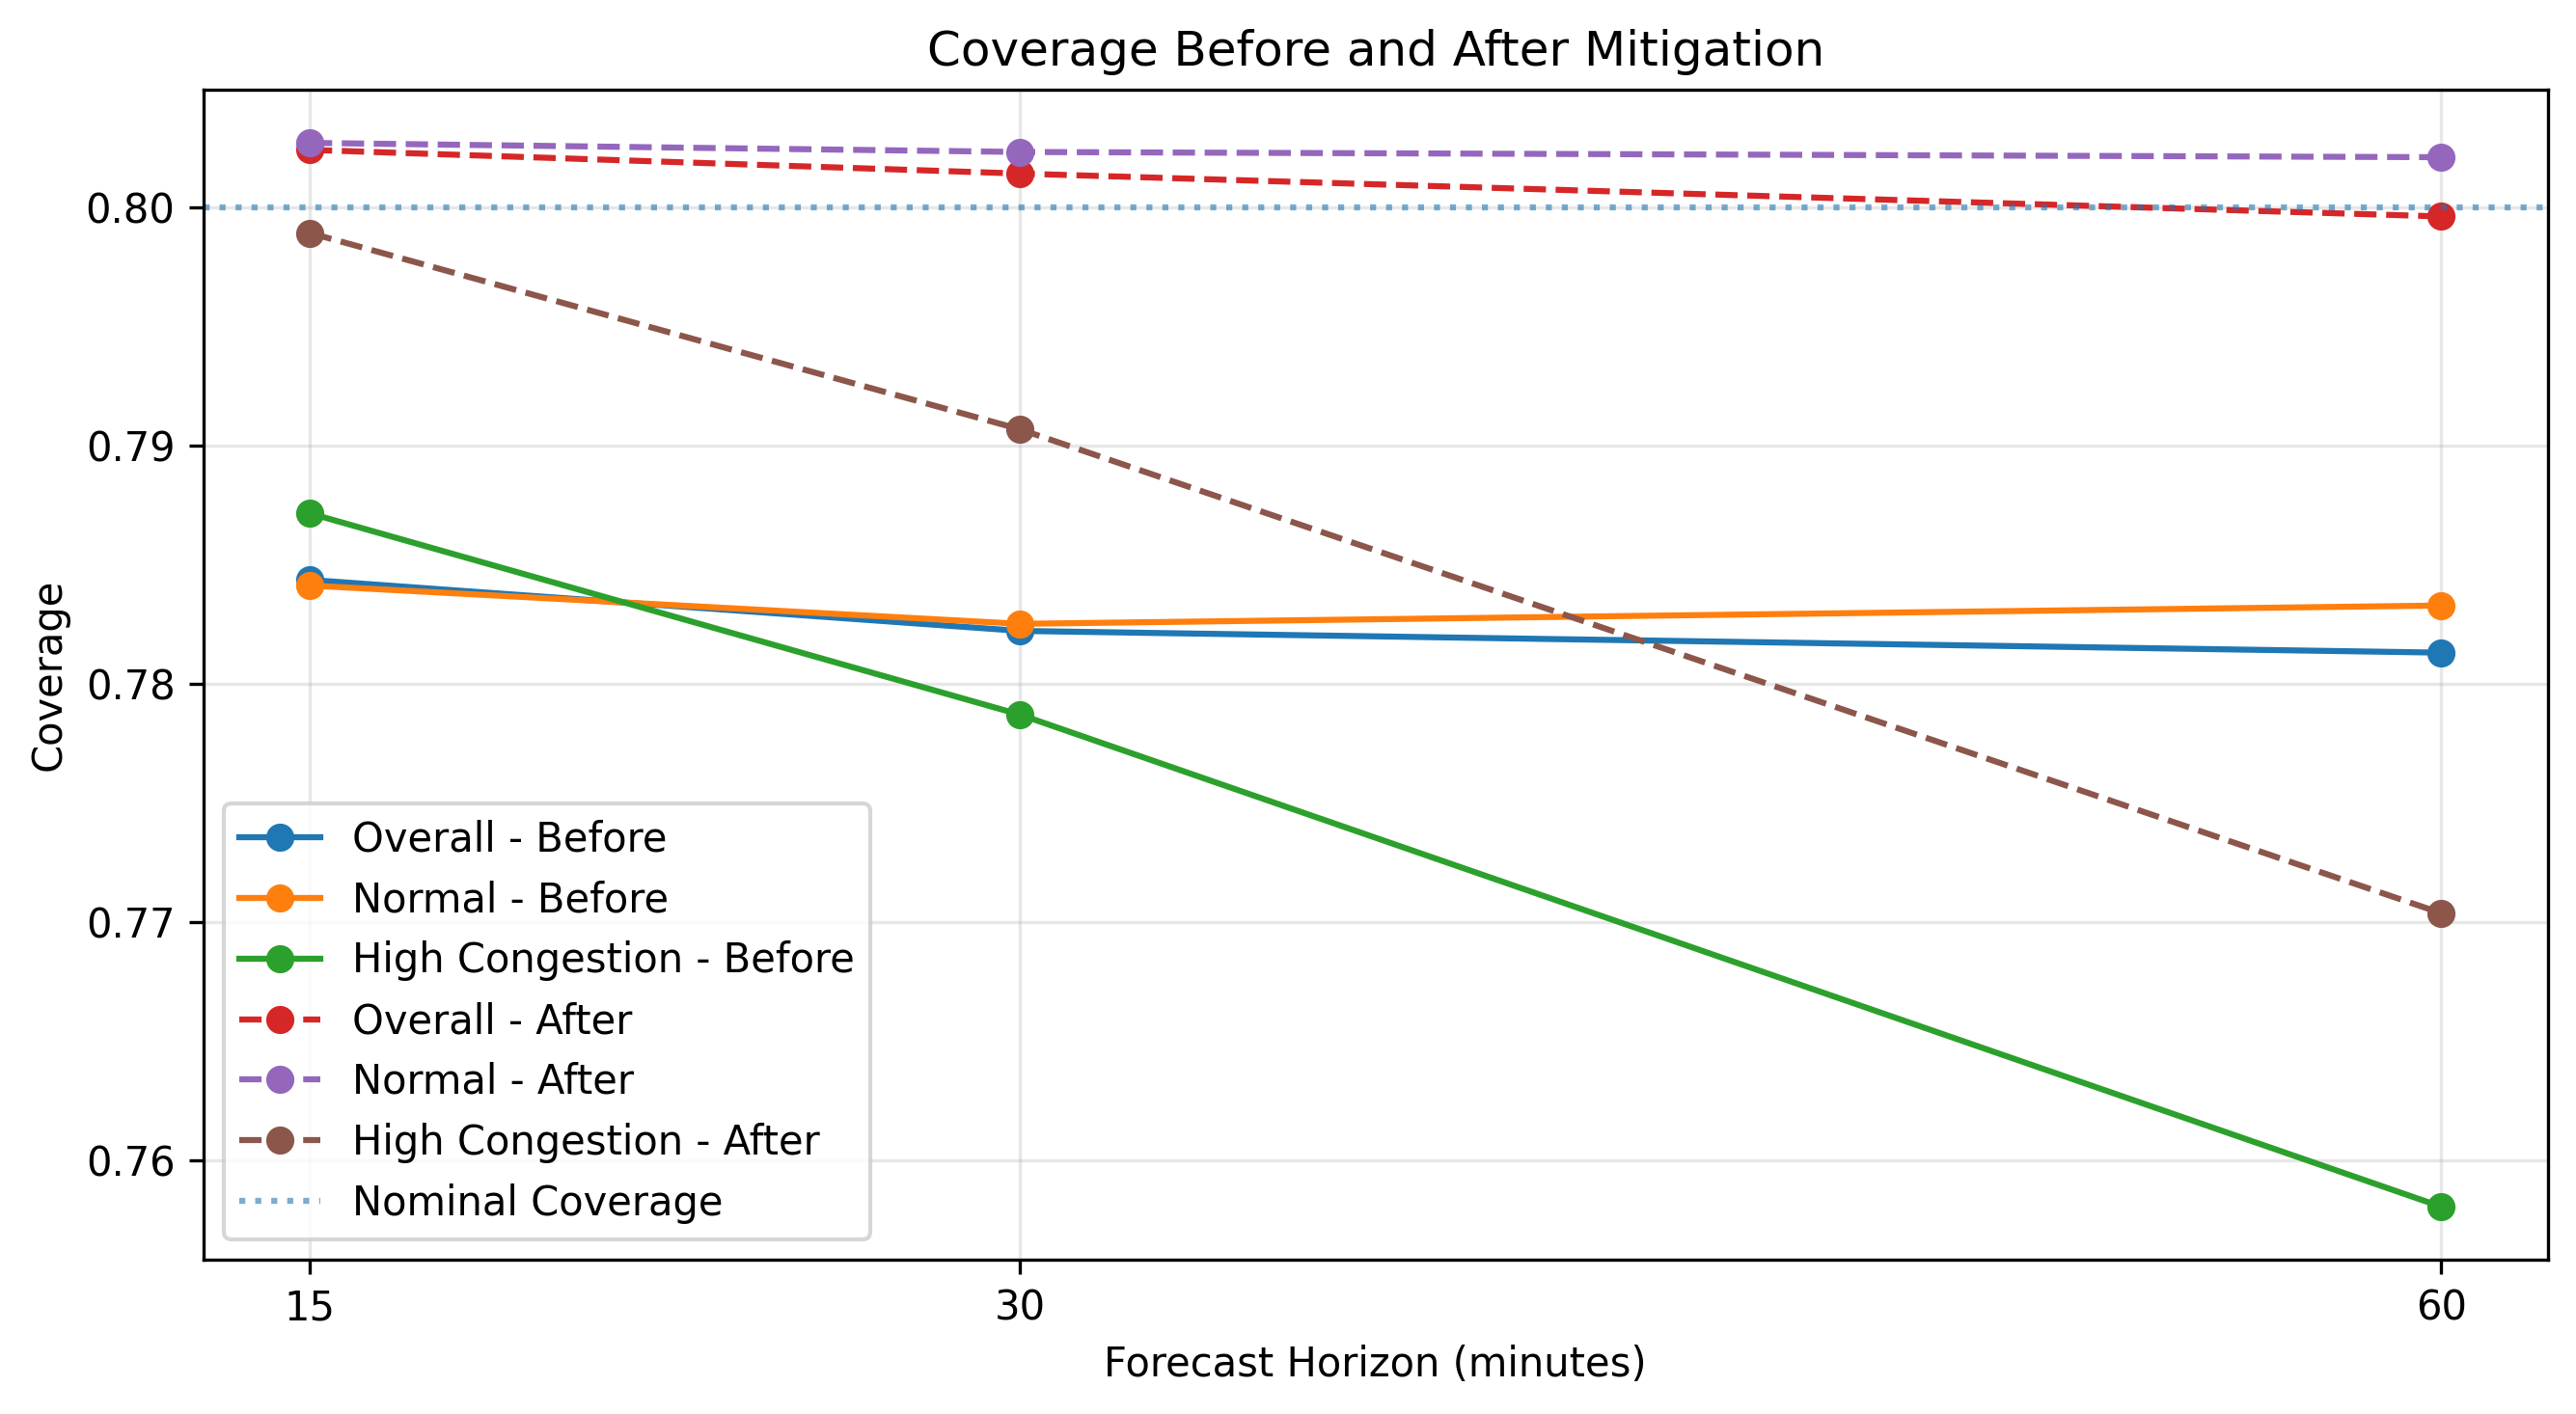
\includegraphics[width=\linewidth]{img/mitigation_strategy/coverage_mitigation_comparison}
    \end{minipage}
    \hfill
    \begin{minipage}[b]{0.49\linewidth}
        \centering
        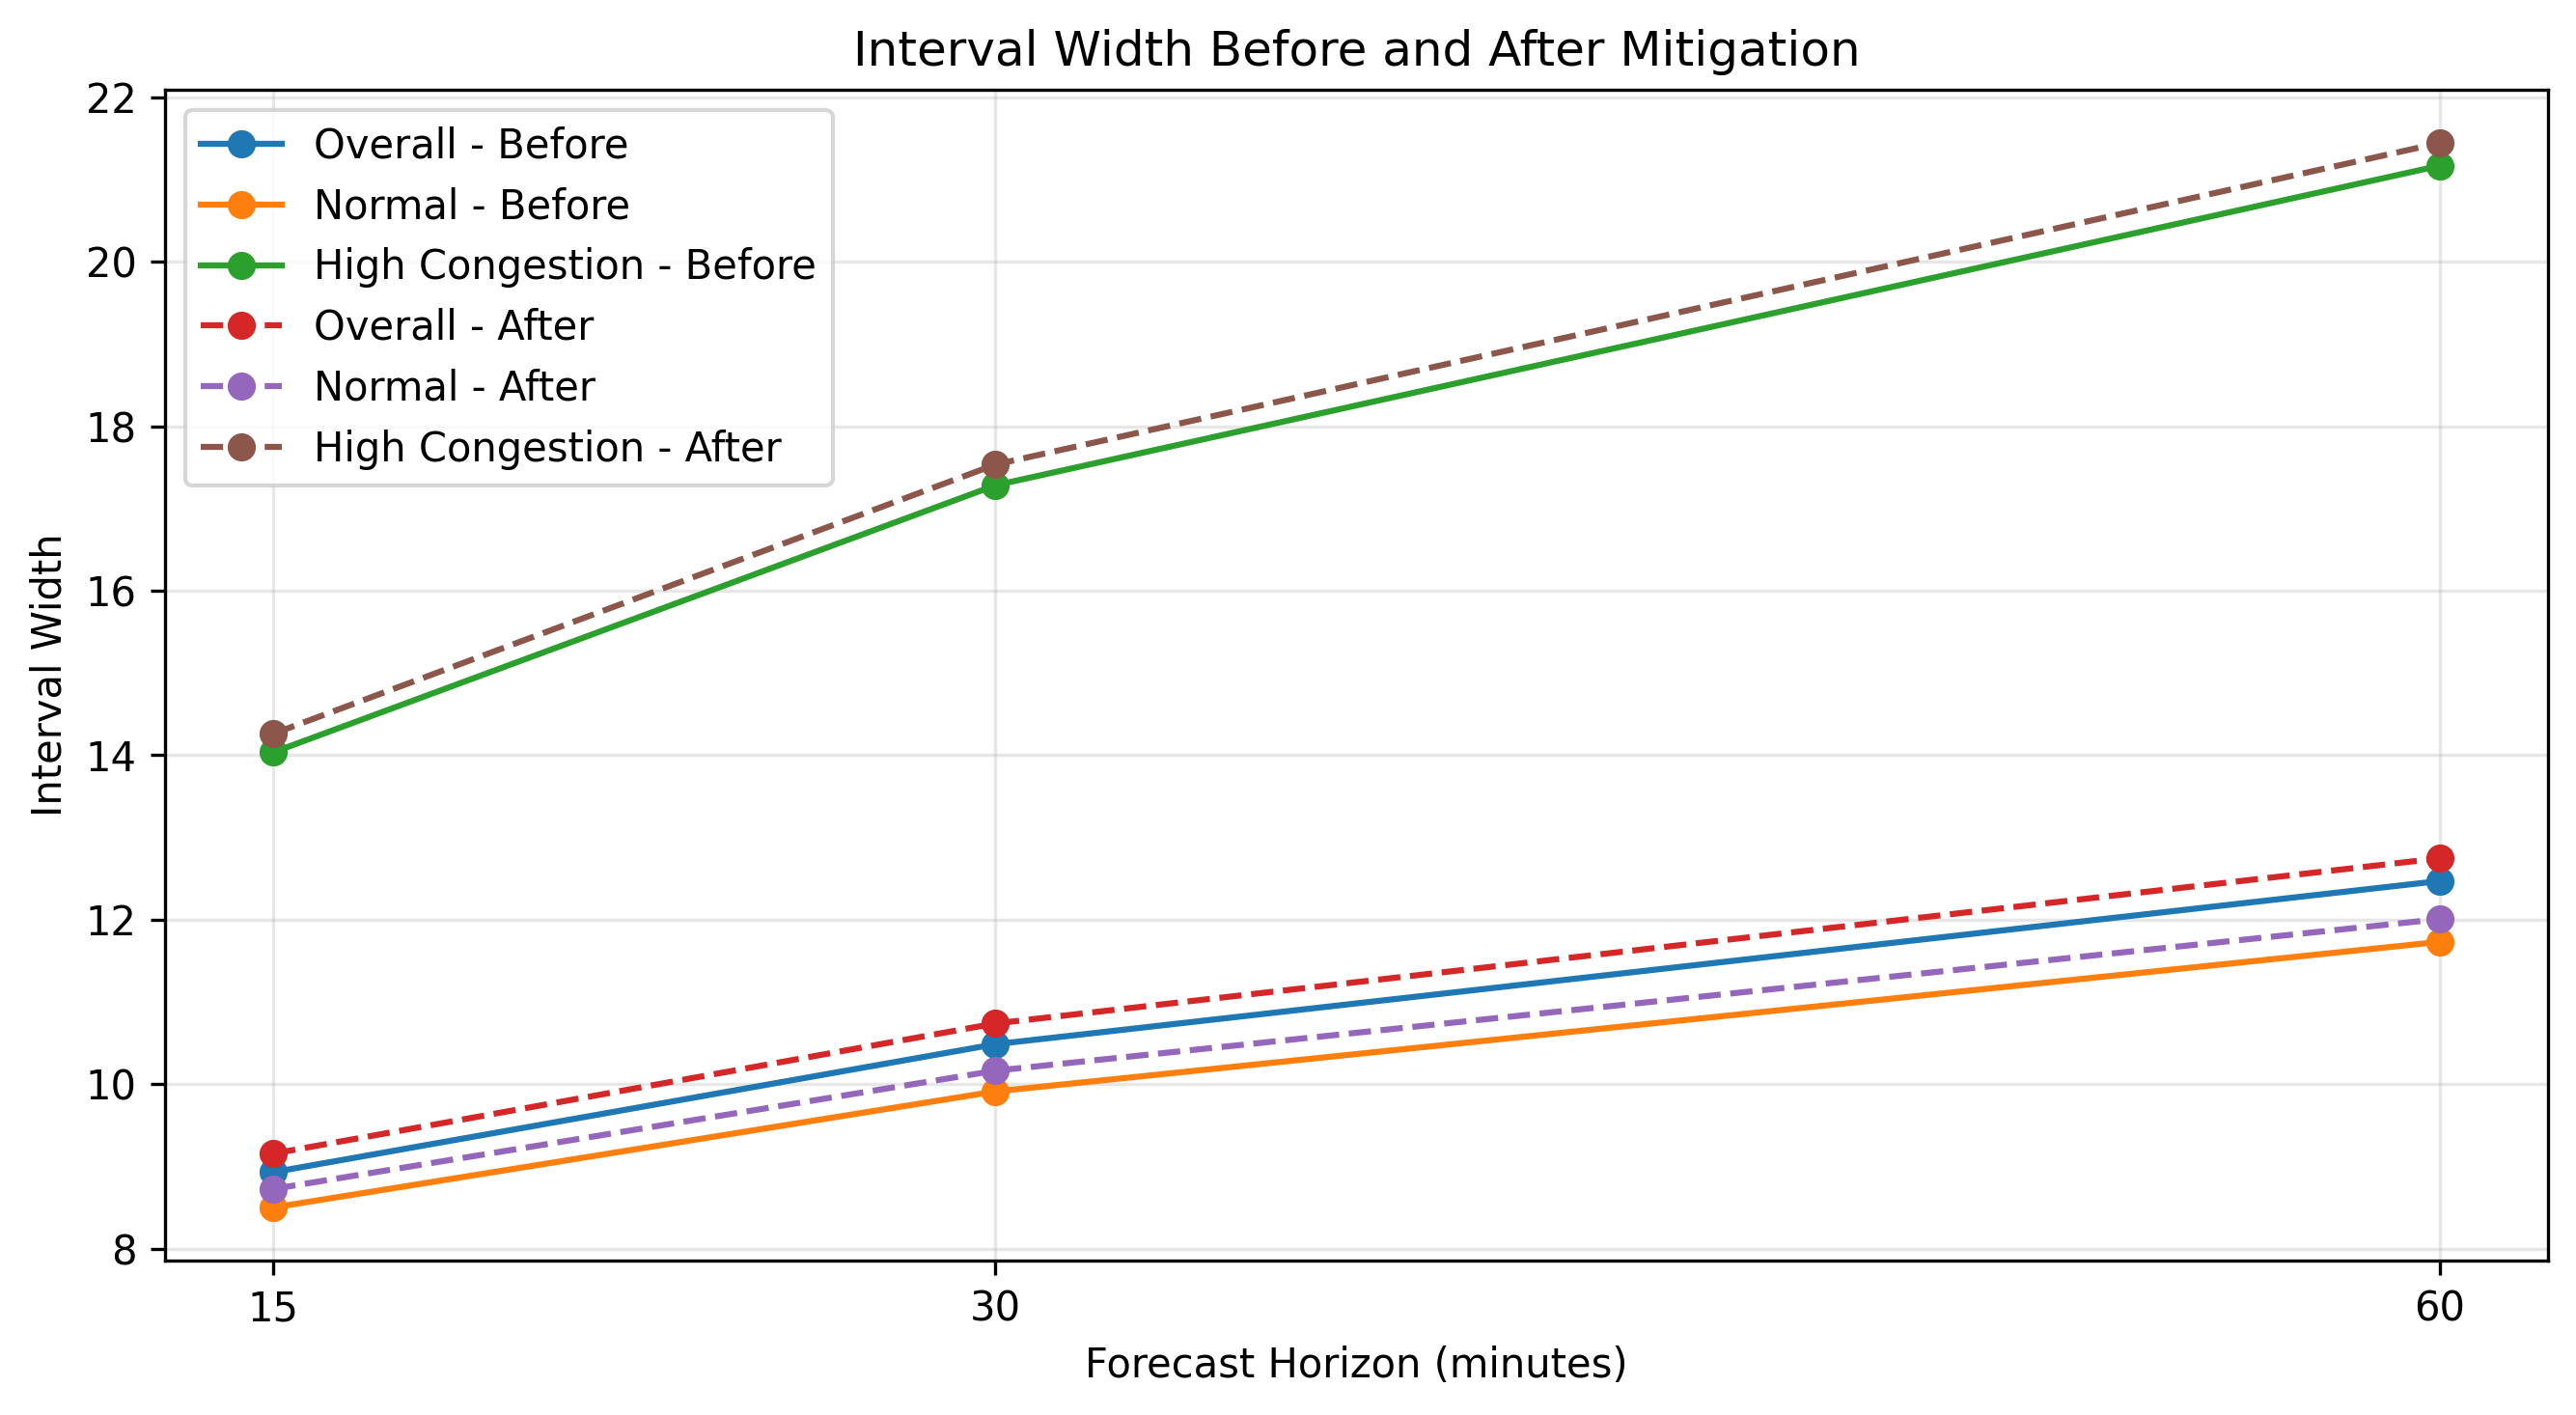
\includegraphics[width=\linewidth]{img/mitigation_strategy/interval_width_mitigation_comparison}
    \end{minipage}

    \caption{Effect of CQR calibration on empirical coverage (left) and
    prediction interval width (right) under overall, normal, and
    high-congestion conditions.}
    \label{fig:cqr_results}
\end{figure}

Figure~\ref{fig:cqr_results} shows that the improvement in coverage is
obtained by moderately expanding the original prediction intervals. Since
CQR leaves the median forecast unchanged, this calibration step improves
uncertainty reliability without altering point forecasting accuracy.

The remaining gap under high congestion, particularly at 60 minutes,
highlights an important limitation of the global calibration strategy.

Overall, CQR successfully mitigates the general undercoverage of the
Graph-Temporal model and substantially improves calibration under normal
conditions. It also improves coverage during high congestion, but does not
completely eliminate the reliability degradation observed at the longest
forecasting horizon. This residual failure motivates considering mitigation
strategies that explicitly account for congestion during model training.


\subsection{Congestion-Aware Training}
\label{subsec:congestion_aware}

Although CQR improves the calibration of the prediction intervals, the
remaining undercoverage under high-congestion conditions suggests that a
global post-hoc correction cannot completely address the distribution shift.
A complementary mitigation strategy would therefore intervene directly
during model training, encouraging the model to allocate greater importance
to observations belonging to congested traffic regimes.

A possible approach is to introduce a congestion-aware weighted version of
the masked Pinball Loss. The congestion condition can be defined using the
same training-derived criterion introduced in
Section~\ref{subsec:congestion_definition}. In particular, each target
timestamp can be associated with its congestion ratio $C_t$, computed using
the per-sensor thresholds estimated exclusively from the training data.

The standard masked Pinball Loss can then be modified by assigning a larger
weight to targets associated with high-congestion conditions. Let
$w_{b,h}$ denote the weight associated with forecasting horizon $h$ of sample
$b$. A simple weighting scheme is

\begin{equation}
    w_{b,h} =
    \begin{cases}
        1 + \lambda, & \text{if } C_{t_b+h} \geq \tau_{\mathrm{peak}}, \\
        1,           & \text{otherwise},
    \end{cases}
    \label{eq:congestion_weight}
\end{equation}

where $\lambda \geq 0$ controls the additional importance assigned to
high-congestion targets. The resulting weighted objective becomes

\begin{equation}
    \mathcal{L}_{\mathrm{weighted}}
    =
    \frac{
        \displaystyle
        \sum_b \sum_h \sum_n
        w_{b,h}\,m_{b,h,n}
        \sum_{q \in \mathcal{Q}}
        \mathcal{L}_q
        \left(
            y_{b,h,n},
            \hat{y}^{(q)}_{b,h,n}
        \right)
    }{
        \displaystyle
        |\mathcal{Q}|
        \sum_b \sum_h \sum_n
        w_{b,h}\,m_{b,h,n}
    }.
    \label{eq:weighted_pinball}
\end{equation}

This modification increases the contribution of congested targets to the
training objective without discarding or undersampling observations from
normal traffic conditions. The hyperparameter $\lambda$ would control the
strength of the reweighting and should be selected using the validation set,
considering both normal and high-congestion performance.

Unlike CQR, which adjusts already estimated prediction intervals, this
strategy would modify the parameters learned by the forecasting model.
Consequently, it could potentially improve both the median forecast and the
estimated conditional quantiles during congestion. This is particularly
relevant to the qualitative behavior observed in
Figure~\ref{fig:shift_examples}, where the high-congestion example exhibits
not only insufficient interval coverage but also a progressively displaced
median forecast at longer horizons.

Importantly, the congestion labels would only be required during training
to construct the weights in Equation~\ref{eq:congestion_weight}. At inference
time, the trained model would continue to receive exactly the same inputs as
the original Graph-Temporal model and would not require knowledge of future
congestion conditions.

This approach was not implemented in the present work and is therefore
proposed as a possible extension rather than evaluated experimentally.
Compared with the post-hoc CQR mitigation, congestion-aware training directly
targets the regime in which the largest degradation was observed. However,
increasing the contribution of relatively rare congestion events may introduce
a trade-off with performance under normal conditions. For this reason, the
weighting strength should be selected carefully and evaluated separately on
normal and high-congestion subsets.

The two mitigation strategies therefore operate at different stages of the
forecasting pipeline. CQR provides a lightweight post-hoc correction that
successfully improves marginal calibration without retraining the model,
whereas congestion-aware training could potentially address the underlying
conditional forecasting errors by explicitly exposing the optimization
objective to the importance of rare congestion regimes.